\documentclass[11pt]{amsbook}
\usepackage[utf8]{inputenc}
\usepackage{Ceyhun}
\usepackage{amsTurkish}

\title{Ceyhun-217}
\author{hkubraeryilmaz }
\date{December 2016}

\begin{document}
\hPage{Ceyhun/217}

Ç(d,a) nın, tümleyeni dışında kalan \textit{kapsar altçizgelerini} düşünelim. $Ç_i$, böylesine bir kapsar altçizgeyi göstersin. Ç(d,a) nın,
\[
    Ç(d,a) = \underset{(i)}{\bigcup} \; Ç_i
\]
biçiminde parçalanmasına, çizgenin \textit{ayrıklarına ayrışması} ve $Ç_i$ altçizgelerine çizgenin \textit{ayrıkları} diyeceğiz.
\
\begin{definition}
    Bütün düğümlerin kertesi n ye eşit olan bir ayrığa, çizgenin \textit{\underline{n-ayrığı}} denir.
\end{definition}

\begin{definition}
    Bütün ayrıkları n-ayrığı olabilecek biçimde ayrışabilen çizgelere, \textit{\underline{n-ayrışır çizge}} denir. 
\end{definition}

Şekil 4.4.1 de, D(8) çizgesinin l-ayrışımı gösterilmiştir. Düğümleri çift sayıya eşit olan dolu çizgelerin l-ayrışırlığı hemen görülebilir. Ayrıca, eşkerteli $\pm (n,n)$ çizgeleri de l-ayrışırdır. 

\begin{wrapfigure}
    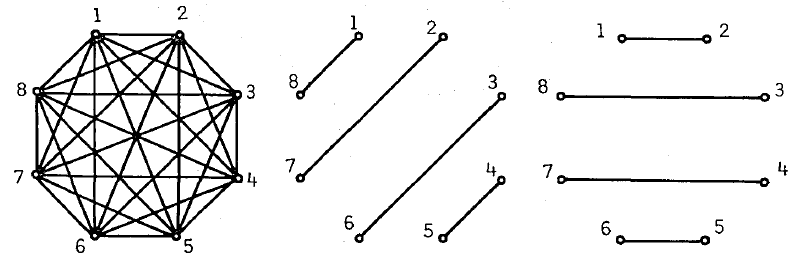
\includegraphics[width=\linewidth]{images/ceyhun-217-fig01.png}
    \caption{}
\end{wrapfigure}

\end{document}